\documentclass[a4paper, 12pt, twppages]{article}

\usepackage[utf8]{inputenc}
\usepackage{amsmath}
\usepackage{amssymb}
\usepackage{enumitem}
%\usepackage{algorithm}
%\usepackage{algorithmic}
%\usepackage{amsfonts}
%\usepackage{latexsym}
\usepackage{bm}
\usepackage{hyperref}
\usepackage{graphicx}
\usepackage{eso-pic}  %% PACKAGE FOR THE BACKGROUNDPIC
\usepackage{fancyhdr}  %% PACKAGE FOR THE HEADERS AND FOOTERS
\usepackage{pdfpages}  %% PACKAGE TO INCLUDE A PDF FILE
\usepackage[round]{natbib}
\usepackage{multirow}
\usepackage{makecell}
\usepackage{textcomp}
\usepackage{floatpag}
\floatpagestyle{empty}

\renewcommand\theadfont{\normalsize}
\newcommand{\comment}[1]{}
\newcommand{\pd}[2]{\frac{\partial #1}{\partial #2}}
\newcommand{\E}[1]{\mathbb{E}\left\{#1\right\}}

\newcommand\BackgroundPic{%
	\put(0,0){%
		\parbox[b][\paperheight]{\paperwidth}{%
			\vfill
			\centering
			
\includegraphics[width=\paperwidth,height=\paperheight,keepaspectratio]{background.pdf}%
			\vfill
		}
	}
}
\fancyhf{}% Clear all headers/footers
%\renewcommand{\headrulewidth}{0pt}% No header rule
%\renewcommand{\footrulewidth}{0pt}% No footer rule
%\fancyfoot[L]{\hspace*{-16mm}\includegraphics[scale=0.3]{logoDepartment.pdf}}

\includeonly{sections/introduction,sections/leverage,sections/model,sections/implementation,sections/computations,sections/results,sections/conclusion}
%\includeonly{sections/02_model}

\let\$\textdollaroldstyle

\begin{document}
	
\includepdf[pages={1}]{scan-of-declaration-of-authorship.pdf}
	\pagebreak
	
	\AddToShipoutPicture*{\BackgroundPic}
	\thispagestyle{fancy}
	
	
	{\vspace{2cm}~}
	{\vspace{2cm}}
	
	%% SELECT BACHELOR OR MASTER THESIS
	{\noindent\large Master Thesis}
	
	
	\vspace{1cm}
	
	%% WRITE THE TITLE OF YOUR WORK
	{\noindent\huge\textbf{Bayesian Estimation of the \\Stochastic Volatility model with \\leverage: \\The case of Germany and China}}
	
	\bigskip
	
	%% WRITE YOUR NAME, date of birth, Student ID
	{\noindent\LARGE Darjus \textsc{Hosszejni}}
	
	%% WRITE YOUR date of birth, Student ID
	\bigskip
	{\noindent\small Date of Birth: August 27, 1991}\newline
	{\noindent\small Student ID: 1551490}
	
	\bigskip
	\bigskip
	\bigskip
	%{\vspace{2cm}}
	{\noindent\large {\bf Subject Area}\\Leverage effect, Bayesian inference}
	
	%% WRITE YOUR Studienkennzahl
	\bigskip
	{\noindent\large {\bf Programme Identification Number}\\J 066 961}
	
	\bigskip
	
	
	%% WRITE THE NAME OF YOUR SUPERVISOR
	{\noindent\large {\bf Supervisor}\\ Mag.rer.soc.oec.~MMag.rer.nat.~Dipl.-Ing.~Dr.techn.\\
		Gregor~\textsc{Kastner}}
	
	\bigskip
	
	%% WRITE THE DATAE OF SUBMISSION
	{\noindent\large {\bf Date of Submission}\\September 9, 2017}
	
	\bigskip\bigskip\bigskip
	
	{\em\noindent Department of Finance, Accounting and Statistics\\
		Vienna University of Economics and Business\\
		Welthandelsplatz 1\\
		1020 Vienna\\
		Austria
	}
	
	
	%\pagestyle{empty}
	\pagebreak
	\tableofcontents
	\pagebreak
	\listoffigures
	\listoftables
	\pagebreak
	
	
	\begin{abstract}
		The Chinese financial market is known to be different from the comparably weakly regulated Western markets in many ways.
    One of the symptoms is the unexpected behaviour observed in Chinese common stocks: their returns and changes in their volatility are not negatively correlated.
    It contrasts an intuitive phenomenon called the leverage effect, which has a history going back even to the 1970s, and it is implied by the assumptions in the popular framework of Modigliani and Miller.
    The leverage effect's importance is reflected by the number of time series models that have been developed for its estimation.
    Although most of them are ARCH-type models, we use a promising alternative called the Stochastic Volatility (SV) model with leverage, that has not been applied to Chinese stock datasets yet, and it has better in-sample-fit than its corresponding, similarly sophisticated GARCH models.
    SV is used in this master thesis for the comparison of the leverage effect observed in Chinese and Western markets.
    As the leading economy of the Eurozone, Germany is chosen to represent the latter.
    Our results show the lack of consistent leverage or anti-leverage effect in China altogether, while they confirm the existence of the leverage effect in Germany.
    As a by-product, we find evidence for the stocks having stronger leverage effect through the crisis of 2007.
	\end{abstract}
	
	\pagebreak
	
	\section{Introduction}

Modelling the variance\footnote{In this document variance means variance of the returns and volatility is the standard deviation of returns.} of the rate of return on stocks is a cornerstone of modern finance.
Variance is a basic building block of risk measurement and prediction uncertainty, and capturing empirical facts about its behaviour is the aim of many theorists~\citep{Christie1982}.
A well-known fact is the seasonality of volatility~\citep{schwert1989why}.
This master thesis is concerned with another empirical fact, the so-called leverage effect, also called asymmetric volatility, that captures the correlation between volatility and return.

\subsection{The anti-leverage effect in China}

The leverage effect is, by definition, the negative relationship between the change in return and the change in volatility.
It was first described by~\citet{black1976studies}, whose explanation was the connection to firms' leverage ratio (LR), i.e. the market equity to debt ratio.
Asymmetric volatility can be deduced in basic structural models of corporate finance~\citep{Christie1982}.
The effect has also been shown using both realised volatility and implied volatility estimates of various models~\citep{Bouchaud2001,Harvey1996,Christie1982,french1987expected}.

The Chinese financial market has been traditionally different from western systems mainly due to the differently regulated environment~\citep{GORDON2003}.
That also leads to counter-intuitive consequences that are not in line with widely used assumptions.
\citet{Shen2009} compared the leverage effect in Germany and in China, and they found a positive correlation between returns and volatility, contradicting the previously mentioned works resulting in negative correlation.


\subsection{Objective}

The main question addressed by this master thesis:
\begin{center}
	Can the Chinese anti-leverage effect be confirmed in different setups?
\end{center}
The question is a reflection to~\citet{Shen2009}, it is answered after choosing an appropriate model that estimates the leverage effect.
As a by-product, a result is acquired about the leverage effect changing consistently in time across firms.
To the best of my knowledge, that question has not been investigated yet in the literature. ???

	\section{Related work}

Variance of stock returns plays an important role in many fields of finance.
For example, it is crucial in capital asset pricing~\citep{skiadas2009asset}, portfolio management~\citep{chow2014study}, and contingent claim pricing~\citep{hull1987pricing}.
\citeauthor{Christie1982} wrote in 1982 that even though volatility was pivotal in these topics, little work was being done for understanding its properties.

This has changed since 1982.
That year~\citet{Engle1982} introduced the Autoregressive Conditional Heteroskestacity (ARCH) model that models non-constant variance conditional on the past.
The ARCH model was later generalised to model volatility more flexibly~\citep{Bollerslev1986}.
Also in 1982, the Stochastic Volatility model was presented in~\citet{Taylor1982}, which models variance as a random process also unconditionally.

aaa

It was first described by~\citet{black1976studies}, who proposed two possible explanations.
The first one, and that is probably where the name comes from, was the connection to firms' leverage ratio, i.e. the market equity to debt ratio.
This theory is underlined by the fact that the existence of the leverage effect can be proved in basic structural models of corporate finance, e.g.~\citeauthor{Christie1982} in the Modigliani--Miller world and some of its generalisations.

The effect has been shown using both realised volatility and implied volatility of various models~\citep{Bouchaud2001,Harvey1996,Christie1982,french1987expected}.

Input of Heston model

\subsubsection{Example from Modiglinani--Miller}

The presence of the phenomenon can also be deduced in widely used structural models of corporate finance, e.g. generalisations of Modigliani--Miller~\citep{Christie1982}.
An illustrating example:  

The leverage effect, definition, illustration, references to its existence, where else is it useful

The leverage effect in Modigliani-Miller and other places

Plots

\subsubsection{Leverage in China}

Leverage in China, references

\subsection{Objective}

Research questions

Possible methods, used method (no formulae)
	\newcommand*{\yts}{y_t^\ast}
\newcommand*{\ets}{\varepsilon_t^\ast}

\section{Model}

The Stochastic Volatility model was introduced in the seminal work of~\citet{Taylor1982}.
By choosing SV, one aims at capturing time varying and seasonal volatility using an AR(1) process.
The model used in this thesis is the Stochastic Volatility with Leverage, which, additional to the AR(1) process, also models the leverage effect by letting the stock return and the increment of the log variance have a constant correlation.

\subsection{Formulation}

The SV model with leverage is, as formulated in~\citet{Omori2007},
\begin{equation}
\begin{alignedat}{2}\label{form:orig_model}
y_t & = \varepsilon_t\exp\left(h_t/2\right), && \quad t=1,\dots,T, \\
h_{t+1} & = \mu+\phi(h_t-\mu)+\eta_t, && \quad t=1,\dots,T-1, \\
\begin{pmatrix}
\varepsilon_t \\
\eta_t
\end{pmatrix}
\bigg\vert\left(\rho,\sigma\right) & \sim\text{ i.i.d. }\mathcal{N}_2\left(\bm{0},\bm{\Sigma}\right), && \quad t=1,\dots,T-1, \\
\varepsilon_T &\sim\mathcal{N}(0,1), \\
\bm{\Sigma} & =
\begin{pmatrix}
1 & \rho\sigma \\
\rho\sigma & \sigma^2
\end{pmatrix},
\end{alignedat}
\end{equation}
where $T$ is the number of time points, the only observed variables are the demeaned log returns, $y_t$.
The return at time $t$ is thus conditionally normally distributed, given $h_t$.
The log variance, $\bm{h}$, is a latent vector, and it constitutes an AR(1) process with mean $\mu$, persistence $\phi$ and variance $\sigma^2$.
Leverage is the fourth parameter, $\rho$, which is the correlation between $\varepsilon_t$ and $\eta_t$, i.e.\ the increment of the stock price and the increment of the log variance.

The first equation in~\eqref{form:orig_model} is not linear in $h_t$, which makes the model difficult to estimate. For the ease of notation, let
\begin{align*}
\yts &=\log(y^2_t), \\
d_t &=I(y_t\ge0)-I(y_t<0), \qquad\text{$y_t$'s sign,} \\
\ets &=\log(\varepsilon^2_t),
\end{align*}
thus knowing $y_t$ is equivalent to knowing the pair $(\yts, d_t)$\footnote{Except for the case $\{y_t=0\}$, which is a null set in the model, and it causes identifiability issues for $h_t$. In practice, we use $\yts =\log(y^2_t+\epsilon)$ with some small $\epsilon$ for robustness.}. By storing $d_t$ and applying $x\mapsto\log(x^2)$ to the first equation of~\eqref{form:orig_model} we get the linearised form,
\begin{align}
\begin{split}\label{form:lin_model}
\yts & = h_t+\ets, \\
h_{t+1} & = \mu+\phi(h_t-\mu)+\eta_t,
\end{split}
\end{align}
where the error term of the first equation has a $\log(\chi_1^2)$ distribution. The observed variable is $\yts$ and $h_t$ is the latent state.

\subsubsection*{Other forms}

The SV model with leverage was formulated differently in~\citet{Jacquier2004}, where $\varepsilon_t$ and $\eta_{t-1}$ are correlated.
A comparison provided in~\citet{yu2005leverage} revealed that model~\eqref{form:orig_model} is more attractive as it is an Euler approximation to the log-normal Ornstein--Uhlenbeck process.
Hence, the method that fits~\eqref{form:orig_model} also fits the corresponding continuous time process with discretely sampled data.
Moreover, in the alternative specification, $y_t$ is not a martingale difference sequence, and $\rho$ has two roles: leverage and the skewness of $y_t\mid y_1,\dots,y_{t-1}$, which makes it more difficult to interpret its value.
Finally, an empirical comparison also showed the model by~\citet{Jacquier2004} to be inferior to~\ref{form:orig_model}.
For these reasons, we use~\eqref{form:orig_model} in the paper at hand.

\subsection{Estimation without leverage}

SV models are an attractive alternative to GARCH type models, the main difference\footnote{For a more in-depth comparison see~\citet{Harvey1994}.} being that while the volatility of GARCH at $t+1$ is conditionally deterministic, given the information known at $t$, it is random in SV.
On the one hand, this lets SV fit the data better in some cases~\citep{Kim1998,kastner2016dealing,Chan2016}, on the other hand, it makes its estimation more difficult. In the following parts, the fitting methods for SV without leverage considered in the literature are briefly summarised.

\subsubsection{Maximum likelihood estimation}

Let $\bm{y}=(y_1,\dots,y_n)$.
In order to obtain an ML estimate for $(\phi,\sigma^2,\rho,\mu)$, we need to evaluate the likelihood function $\ell(\phi,\sigma^2,\rho,\mu\mid\bm{y})$, for which we need to integrate over the space of vector $\bm{h}$.
This is unfortunately difficult due to the non-linear dependence between $y_t$ and $h_t$, or, in the linear form, due to the non-Gaussian error term $\ets$.

The issue of non-normality was resolved in~\citet{Harvey1994} using a Gaussian approximation to $\ets$, i.e.\ by matching the first two moments of the $\log(\chi_1^2)$ distribution.
Then, in the resulting approximate model, using a Kalman filter to integrate over $\bm{h}$, a quasi-likelihood function can be calculated, and, after maximisation, a quasi-maximum likelihood estimate can be obtained.
This estimator is consistent and asymptotically normally distributed, but it has bad performance in small samples because the $\ets$ is poorly approximated by the normal distribution~\citep{Kim1998}.

\subsubsection{Bayesian approach}

The lack of a closed form likelihood function also means that there are no closed form posteriors for the model.
This suggests the usage of Markov chain Monte Carlo algorithms (MCMC), which, with the help of Markov chains and Bayes' theorem, make it possible to draw samples from the posterior distribution of the latent variables and the parameters.
With enough such samples we get a picture of these distributions.
For an introduction, see, e.g.,~\citet{Geyer2011} or Section~\ref{sec:estimlev} of the paper at hand.

In~\citet{Kim1998}, two different Bayesian ideas were compared for SV without leverage based on how the latent variables are sampled.
A single move (one-at-a-time volatility update) sampler was introduced first. It draws $h_t$ from $h_t\mid\bm{h}_{-t},\bm{y},\phi,\sigma^2,\mu$ one by one, where $\bm{h}_{-t}$ is $\bm{h}$ excluding $h_t$.
Due to the high intercorrelation in $\bm{h}$, slow convergence and poor mixing characterise this approach even though the algorithm used by~\citet{Kim1998} performs better than the other ones in the literature~\citep{shephard1993fitting,jacquier2002bayesian,shephard1994comment,shephard1997likelihood,geweke1994bayesian}.

To avoid the issues with high intercorrelation in $\bm{h}$, a multi-move sampler was used that draws $\bm{h}$ from $\bm{h}\mid\bm{y},\phi,\sigma^2,\mu$ at once.
By approximating the marginal distribution of $\ets$ with a $K=7$ component mixture of normals,~\citet{Kim1998} managed to reduce the task to the known framework of conditionally Gaussian state spaces\footnote{For an introduction see~\citet{Kitagawa1996}.}.
Since the marginal of $\ets$ does not include any model-dependent values, this mixture of normals can be specified before fitting the model.
The approximation errors to the original SV model can be corrected for by a reweighting scheme.
However, this correction is known to have minor influence due to the good choice of the mixture approximation~\citep{Kim1998}.

\subsection{Approximate model}

Both the single move and the multi-move samplers were generalised to SV with leverage in~\citet{Omori2007}, and a particle filtering\footnote{For an introduction see~\citet{Johannes2009}.} method was also derived.
In this work, we favor MCMC methods over sequential Monte Carlo (particle filtering) due to the availability of computers with a multitude of strong processors.
Finally, due to its better sampling efficiency, the multi-move sampler was chosen over the single move sampler for fitting the model.

\subsubsection{Bivariate normal approximation}

Due to the correlation between $\varepsilon_t$ and $\eta_t$, approximating $\ets$ affects $\eta_t$ as well.
Thus,~\citet{Omori2007} used a mixture of bivariate normals as an approximation to the conditional distribution of the pair $(\ets, \eta_t)$.
Let $(\xi_t,\nu_t\mid d_t,\rho,\sigma)$ denote the approximate random variable to $(\ets,\eta_t\mid d_t,\rho,\sigma)$, and let $\pi(X)$ denote the density of the random variable $X$ and $\pi(X=x)$ denote its value at $x$.

In order to derive the approximation, we first decompose the bivariate conditional density and then approximate the parts separately,
\begin{align}
\pi(\ets,\eta_t\mid d_t,\rho,\sigma) &= \pi(\ets\mid d_t,\rho,\sigma)\cdot \pi(\eta_t\mid\ets,d_t,\rho,\sigma),\nonumber \\
&= \pi(\ets)\cdot \pi(\eta_t\mid\ets,d_t,\rho,\sigma)\label{eq:decomp},
\end{align}
because the marginal of $\ets$ is independent of $d_t$, $\rho$, and $\sigma$.
\citet{Omori2007} now used an improved normal mixture approximation to the marginal $\pi(\ets)$ with $K=10$,
\begin{equation}\label{eq:ets}
\pi(\xi_t)\triangleq\sum_{j=1}^{10}p_j\pi\left(\mathcal{N}\left(m_j,v_j^2\right)\right),
\end{equation}
where $\pi\left(\mathcal{N}\left(m_j,v_j^2\right)\right)$ denotes the normal density with mean $m_j$ and variance $v_j^2$.
The constants $m_j$, $p_j$ and $v_j$ are specified in Table~\ref{tab:constants}.

The conditional distribution of $\eta_t$ is
\begin{equation*}
\eta_t\mid\ets,d_t,\rho,\sigma\sim\mathcal{N}\left(d_t\rho\sigma\exp(\ets/2),\sigma^2\left(1-\rho^2\right)\right),
\end{equation*}
thus, we could use
\begin{equation}\label{eq:eta}
\nu_t\mid\xi_t,d_t,\rho,\sigma\sim\mathcal{N}\left(d_t\rho\sigma\exp(\xi_t/2),\sigma^2\left(1-\rho^2\right)\right),
\end{equation}
but the term $\exp(\xi_t/2)$ introduces difficulties.
These are mitigated by a linear approximation
\begin{equation}\label{eq:etslinear}
\exp(\xi_t/2)\approx\exp(m_j/2)(a_j+b_j(\xi_t-m_j))
\end{equation}
when the $j$th mixture component is used for $\xi_t$, i.e.\ $\mathcal{N}(m_j,v_j^2)$.
The constants $a_j$ and $b_j$ were found by minimising the mean square norm 
\begin{equation*}
\E{\left[\exp(\xi_t/2)-\exp(m_j/2)(a+b(\xi_t-m_j))\right]^2}
\end{equation*}
w.r.t. $a$ and $b$, separately for each $j$, and they are listed in Table~\ref{tab:constants}.

\begin{table}[h!]
	\centering
	\caption{Constants of the bivariate approximation~\citep{Omori2007}.}
	\label{tab:constants}
	\begin{tabular}{cccccc}
		$j$                       & $p_j$    & $m_j$      & $v_j^2$ & $a_j$    & $b_j$    \\ \hline
		\multicolumn{1}{l|}{1}  & 0.00609 & 1.92677   & 0.11265                & 1.01418 & 0.50710 \\
		\multicolumn{1}{l|}{2}  & 0.04775 & 1.34744   & 0.17788                & 1.02248 & 0.51124 \\
		\multicolumn{1}{l|}{3}  & 0.13057 & 0.73504   & 0.26768                & 1.03403 & 0.51701 \\
		\multicolumn{1}{l|}{4}  & 0.20674 & 0.02266   & 0.40611                & 1.05207 & 0.52604 \\
		\multicolumn{1}{l|}{5}  & 0.22715 & -0.85173  & 0.62699                & 1.08153 & 0.54076 \\
		\multicolumn{1}{l|}{6}  & 0.18842 & -1.97278  & 0.98583                & 1.13114 & 0.56557 \\
		\multicolumn{1}{l|}{7}  & 0.12047 & -3.46788  & 1.57469                & 1.21754 & 0.60877 \\
		\multicolumn{1}{l|}{8}  & 0.05591 & -5.55246  & 2.54498                & 1.37454 & 0.68728 \\
		\multicolumn{1}{l|}{9}  & 0.01575 & -8.68384  & 4.16591                & 1.68327 & 0.84163 \\
		\multicolumn{1}{l|}{10} & 0.00115 & -14.65000 & 7.33342                & 2.50097 & 1.25049
	\end{tabular}
\end{table}

By combining~\eqref{eq:decomp},~\eqref{eq:ets},~\eqref{eq:eta} and~\eqref{eq:etslinear}, we get the final approximation
\begin{align*}
\pi(\ets,\eta_t\mid d_t,\rho,\sigma) &\approx \pi(\xi_t,\nu_t\mid d_t,\rho,\sigma), \\
&= \pi(\xi_t)\cdot \pi(\nu_t\mid\xi_t,d_t,\rho,\sigma), \\
&= \sum_{j=1}^{10}p_j\pi(\mathcal{N}\left(m_j,v_j^2\right))\cdot \\
&\quad\cdot\pi\left(\mathcal{N}\left(d_t\rho\sigma\exp(m_j/2)(a_j+b_j(\xi_t-m_j)),\sigma^2\left(1-\rho^2\right)\right)\right).
\end{align*}

\subsubsection{Correcting for misspecification}\label{sec:reweight}

Let $\theta$ denote $(\sigma,\rho,\phi)$.
By using an approximate distribution for the true $\pi(\ets,\eta_t\mid d_t,\rho,\sigma)$, we misspecified the model, and our draws for $\bm{h}$, $\theta$ and $\mu$ are from an approximate posterior density as well.
One can correct this and produce draws from the true posterior $\pi(\bm{h},\theta,\mu\mid\bm{y})$ by calculating weights $w_k$, for all the draws $k=1,\dots,N$, and resample the sampled numbers according to the weights.
After obtaining the error terms
\begin{align*}
\xi_t^k &= y_t^\ast-h_t^k, \\
\nu_t^k &= (h_{t+1}^k-\mu^k)-\phi^k(h_t^k-\mu^k).
\end{align*}
Then, we compute the non-normalised weights
\begin{equation*}
w_k^\ast=\frac{\pi\left(\ets=\xi_t^k,\eta_t=\nu_t^k\mid d_t,\mu=\mu^k,\theta=\theta^k\right)}{\pi\left(\xi_t=\xi_t^k,\nu_t=\nu_t^k\mid d_t,\mu=\mu^k,\theta=\theta^k\right)},
\end{equation*}
Finally, we normalise the weights
\begin{equation*}
w_k=\frac{w_k^\ast}{\sum_{l=1}^{T}w_l^\ast}
\end{equation*}
to get the probabilities that we use for resampling the existing draws.
\citet{Omori2007} found that the weights have quite small variance which makes the effect of this correction procedure modest.
That is in line with the demonstrated high precision of the approximate bivariate distribution.

\subsubsection[State space form]{Conditional Gaussian state space form}

Due to the normal mixture approximation, a new variable $\bm s=(s_1,\dots,s_T)$ has been introduced to the model, the vector of mixture components, one component for each time point. Given $s_t=j$, we end up with a linear model with normal errors,
\begin{equation}
\begin{alignedat}{2}\label{form:appr_model}
\yts & = h_t+\xi_t, && \quad t=1,\dots,T, \\
h_{t+1} & = \mu+\phi(h_t-\mu)+\nu_t, && \quad t=1,\dots,T-1, \\
\begin{pmatrix}
\xi_t \\
\nu_t
\end{pmatrix} &\overset{d}{=}
\begin{pmatrix}
m_j \\
a_j\gamma_t^j
\end{pmatrix} +
\begin{pmatrix}
v_j && 0 \\
b_jv_j\gamma_t^j && \sigma\sqrt{1-\rho^2}
\end{pmatrix}
\begin{pmatrix}
z_t^1 \\
z_t^2
\end{pmatrix}, && \quad t=1,\dots,T-1, \\
\xi_T &\overset{d}{=} m_j+v_jz_t^1, \\
\begin{pmatrix}
z_t^1 \\
z_t^2
\end{pmatrix}
&\sim\text{ i.i.d. }\mathcal{N}_2\left(\bm{0},\bm{I_2}\right), && \quad t=1,\dots,T,
\end{alignedat}
\end{equation}
where $\gamma_t^j\triangleq d_t\rho\sigma\exp(m_j/2)$ and ``$\overset{d}{=}$'' means equivalence in distribution. Note that $(\xi_t,\nu_t)$ depends on $d_t,\rho,\sigma$ and $s_t$.

In order to reduce the estimation of model~\eqref{form:appr_model} to the estimation of a well-known framework, we reformulate the first two equations of~\eqref{form:appr_model} equivalently as
\begin{equation}
\begin{alignedat}{2}\label{form:gauss_model}
\begin{pmatrix}
\yts \\
h_{t+1} \\
\tilde{\mu}_{t+1}
\end{pmatrix} &=
\begin{pmatrix}
h_t \\
\tilde{\mu}_t+\phi(h_t-\tilde{\mu}_t) \\
\tilde \mu_t
\end{pmatrix} +
\begin{pmatrix}
\xi_t \\
\nu_t \\
0
\end{pmatrix}, \quad t=1,\dots,T-1, \\
y_T^\ast &= h_T+\xi_T.
\end{alignedat}
\end{equation}
Since $(\xi_t,\nu_t,0)$ is a (degenerate) normal white-noise series, setting $\mu\equiv\tilde{\mu}_t$ and assuming a normal prior for $\mu$ and $h_1\mid(\mu,\sigma,\phi)$, model~\eqref{form:gauss_model} is a linear Gaussian state space (GSS) with hidden state $(h_t,\tilde{\mu}_t)$.
We copy the priors of the initial latent state used by~\citet{Omori2007}, for arbitrary constant $\sigma_0$,
\begin{equation*}
\begin{pmatrix}
h_1 \\
\tilde\mu_1
\end{pmatrix} \sim
\mathcal{N}\left(
\begin{pmatrix}
\mu_0 \\
\mu_0
\end{pmatrix},
\begin{pmatrix}
\sigma^2/(1-\phi^2)+\sigma_0^2 & \sigma_0^2 \\
\sigma_0^2 & \sigma_0^2
\end{pmatrix}
\right).
\end{equation*}
Note that in~\eqref{form:gauss_model} $\tilde{\mu}_t$ is constant through $t$. \citet{Omori2007} needed this ``trick'' with the inclusion of $\mu$ in the hidden state in order to match the general form of models that can be fitted via the method in~\citet{de1995simulation}.

\subsection{Estimation with leverage}\label{sec:estimlev}

\subsubsection[MCMC algorithms]{Markov Chain Monte Carlo algorithms}

The term Monte Carlo is used for the simulation of random processes, while the term Markov chain denotes sequences of random variables $X_1,X_2,\dots$ for which, for each $n\in\mathbb{N}$, the conditional distribution of $X_{n+1}$ given $X_1,\dots,X_n$ only depends on $X_n$ (it is ``memoryless'').
This way, the value of $X_n$ can be thought of as the state of the chain at time $n$, and then $f_{X_{n+1}\mid X_n}(v\mid u)$ is the probability or density of transition from state $u$ to state $v$ at time $n$.
Under sufficient conditions, the states of a Markov chain converge in distribution to $\pi$, called the equilibrium distribution, from every initial state having positive density~\citep{grinstead2012introduction}.

In practice, we cannot prove the conditions for the existence of $\pi$.
Instead we only have the output of the algorithm, a sequence of realisations, from which we can try to imply that we have a converged chain using, e.g., visualisations and autocorrelation functions.
\citet{Geyer2011} mentions the issues that pop up here and argues about some solution ideas.

\comment{
	These transition probabilities are called stationary if they don't depend on $n$.
	
	For the majority of the Markov chain Monte Carlo (MCMC) algorithms stationary transition probability distributions are needed.
	These are easier to handle, e.g. the joint distribution of such a Markov chain is characterised by the initial distribution of $X_1$ and on the general transition distribution from $X_n$ to $X_{n+1}$.
	
	The sequence $X_1,X_2,\dots$ itself is called stationary if for each $k\in\mathbb{N}$ and $n\in\mathbb{N}$ the joint distribution of the tuple $(X_n,\dots,X_{n+k})$ is independent of $n$.}

\subsubsection{Steps overview}

After initialising all the latent variables and parameters, there are three main steps when doing a Bayesian estimation of a conditional linear GSS.
\begin{enumerate}[start=0]
	\item Initialise $\bm h,\bm s,\theta,\mu$,
	\item Draw $\bm{s}\mid\bm{y}^\ast,\bm{d},\bm{h},\mu,\theta$\label{enum:draw-s},
	\item Draw $\theta,\bm h,\mu\mid\bm y^\ast,\bm d,\bm s$\label{enum:draw-other},
	\begin{enumerate}
		\item Draw $\theta\mid\bm{y}^\ast,\bm{d},\bm s$\label{enum:draw-theta},
		\item Draw $\bm{h},\mu\mid\bm{y}^\ast,\bm{d},\theta,\bm s$\label{enum:draw-latent},
	\end{enumerate}
	\item Goto Step~\ref{enum:draw-s}.
\end{enumerate}
Steps~\ref{enum:draw-s} and~\ref{enum:draw-other} are interchangeable in the algorithm but~\ref{enum:draw-theta} and~\ref{enum:draw-latent} are not because the former's by-products are needed for the latter.
The steps are detailed below based on~\citet{Omori2007}.

If the Markov chain specified by the algorithm above has an equilibrium distribution, then it is an approximation to $\bm h,\bm s,\theta,\mu\mid\bm y$, the posterior distribution of the parameters and latent variables, and it is the true one after the reweighting scheme (Section~\ref{sec:reweight}).
So by repeating the steps sufficiently many times, after ``reaching convergence'' we obtain draws from the posterior.
With such a sample we can estimate the posterior mean or any other point estimate, calculate credible intervals or transforms of the distribution.

\subsubsection{Drawing the mixture states}

This is the easiest part because we can derive the posterior probabilities $\pi(s_t=j\mid\bm{y},\bm{h},\mu,\sigma,\rho,\phi)$, $j=1,\dots,K$, directly.
We define
\begin{align*}
\hat\xi_t &\triangleq y_t^\ast-h_t, \\
\hat{\nu}_t &\triangleq h_{t+1}-\mu-\phi(h_t-\mu), \\
\gamma_t^j &\triangleq d_t\rho\sigma\exp(m_j/2),
\end{align*}
then, based on~\citet{Omori2007} with $K=10$, for $t=1,\dots,T-1$ and $j=1,\dots,10$,
\begin{equation}
\begin{aligned}[1]
\pi\left(s_t=j\mid\bm{y},\bm{h},\mu,\theta\right) &\propto P\left(s_t=j\right)\cdot\pi\left(\xi_t=\hat\xi_t\mid s_t=j\right)\cdot \\
&\quad\cdot\pi\left(\nu_t=\hat\nu_t\mid\xi_t=\hat\xi_t,s_t=j,h_{t+1},h_t,\mu,\theta\right), \\
\pi\left(s_T=j\mid\bm{y},\bm{h},\mu,\theta\right)
&\propto P\left(s_T=j\right)\cdot\pi\left(\xi_T=\hat\xi_T\mid s_T=j\right)\cdot 1,
\end{aligned}
\end{equation}
where
\begin{align*}
P\left(s_t=j\right) &= p_j, \\
\pi\left(\xi_t=\hat\xi_t\mid s_t=j\right) &\propto \frac{1}{v_j}\exp\left(-\frac{\left(\hat\xi_t-m_j\right)^2}{2v_j^2}\right),
\end{align*}
and
\begin{multline*}
\pi\left(\nu_t=\hat\nu_t\mid\xi_t=\hat\xi_t,s_t=j,h_{t+1},h_t,\mu,\theta\right) \propto \\
\propto \exp\left(-\frac{\left(\hat{\nu}_t-\left(\gamma_t^j\left[a_j+b_j\left(\hat\xi_t-m_j\right)\right]\right)\right)^2}{2\sigma^2\left(1-\rho^2\right)}\right).
\end{multline*}
This way we get values that are just proportional to the posterior probabilities, hence we have to normalise these values so that they sum to 1.
We can use the inverse sampling method to draw $\bm s\mid\bm{y},\bm{h},\mu,\sigma,\rho,\phi$~\citep{grinstead2012introduction}.

\subsubsection{Drawing $\rho,\sigma,\phi$}

The remaining two steps are more involved and based on~\citet{de1995simulation}.
They are detailed and derived for SV with leverage in~\citet{Nakajima2009}, where SV with leverage is extended and it features jumps and t distributed residuals.

In this step, the Metropolis-Hastings (MH) algorithm is used to obtain a draw from $\theta\mid\bm{y}^\ast,\bm{d},\bm s$.
Three things are needed for MH,
\begin{itemize}
	\item Calculate the true density $\pi(\theta\mid\bm{y}^\ast,\bm{d},\bm s)$ up to a constant factor,
	\item A proposal density $g(\theta\mid\bm{y}^\ast,\bm{d},\bm s)$ whose support is a superset of the true support,
	\item A proposed new $\theta_\ast$ from $g(\theta\mid\bm{y}^\ast,\bm{d},\bm s)$.
\end{itemize}
It is important that the evaluation of and sampling from the proposal density is efficient.
Bayes' theorem helps with the first point by decomposing the posterior into the likelihood and the prior: $\pi(\theta\mid\bm{y}^\ast,\bm{d},\bm s)\propto\pi(\bm{y}^\ast\mid\theta,\bm{d},\bm s)\pi(\theta)$.
The likelihood can be computed using the Kalman filter, the prior is usually chosen to be from a well-known family.

Given everything above, a MH step in the $n$th loop
\begin{enumerate}
	\item Produces a candidate $\theta_\ast$ from $g(\theta\mid\bm{y}^\ast,\bm{d},\bm s)$.
	\item The new sample will be either the current value $\theta_n$ or the candidate $\theta_\ast$. The so-called acceptance ratio drives the decision:
	\begin{equation*}
	\text{AR}=\frac{\pi(\bm{y}^\ast\mid\theta_\ast,\bm{d},\bm s)\pi(\theta_\ast)}{\pi(\bm{y}^\ast\mid\theta_n,\bm{d},\bm s)\pi(\theta_n)}\frac{g(\theta_n\mid\bm{y}^\ast,\bm{d},\bm s)}{g(\theta_\ast\mid\bm{y}^\ast,\bm{d},\bm s)}
	\end{equation*}
	\item Finally, $\theta_\ast$ is accepted with probability $\min\left\{\text{AR},1\right\}$, and $\theta_{n+1}=\theta_\ast$.
	Otherwise $\theta_{n+1}=\theta_n$ is the new state again.
\end{enumerate}

\citet{Nakajima2009} chose the proposal to be $\mathcal{N}(c, C)$ truncated to the region $R=\left\{(\sigma,\rho,\phi)\mid\sigma>0,-1<\rho<1,-1<\phi<1\right\}$.
The mean vector $c$ and the covariance matrix $C$ are calculated in each loop in a way that the proposal's log density is the second order Taylor expansion of the true log density around the true log density's mode.\footnote{
	Even though we can only evaluate the true posterior density up to a (positive) constant factor, this works here because the mode is the same, and we differentiate the log density for the Taylor expansion, i.e.\ constant multipliers vanish.}
More precisely,
\begin{align*}
c &= \hat{\theta}+Cv, \\
C^{-1} &= -\frac{\partial^2\log\pi(\theta\mid\bm{y}^\ast,\bm{d},\bm s)}{\partial\theta\partial\theta^\prime}, \\
v &= \frac{\partial\log\pi(\theta\mid\bm{y}^\ast,\bm{d},\bm s)}{\partial\theta}, \\
\hat{\theta} &= \text{arg}\max_\theta\pi(\theta\mid\bm{y}^\ast,\bm{d},\bm s).
\end{align*}

\subsubsection{Drawing $\mu$ and the log variance}

Both $\mu$ and $\bm h$ are sampled using by-products of the Kalman filter used when calculating $\pi(\bm{y}^\ast\mid\theta_{n+1},\bm{d},\bm s)$ for the AR.
The new value of $\mu$ comes by simply drawing from $\mathcal{N}(q_{T+1},Q_{T+1})$, where $q_{T+1}$ and $Q_{T+1}$ are readily available at this point.
In order to get the latent vector $\bm h$, we first sample $\bm{\nu}\mid\bm{y}^\ast,\bm{d},\theta,\bm s$ using a Gaussian simulation smoother~\citep{fruhwirth1994data,carter1994gibbs} and then reconstruct $\bm h$ from the formulas in~\citet{de1995simulation}.

%%%%%%%%%%%%%%%%%%%%%%%%%%%%%%%%%%%%%%%%%%%

\comment{
	\begin{align}
	\pi(s_t=j\mid\bm{y},\bm{h},\mu,\theta)
	&= \pi(s_t=j\mid\bm{y^*},\bm{d},\bm{h},\mu,\theta),\nonumber \\
	&\overset{(1)}{=} \pi(s_t=j\mid y^*_t,d_t,h_{t+1},h_t,\mu,\theta),\nonumber \\
	&\overset{(2)}{=} \pi(s_t=j\mid \xi_t,d_t,\nu_t,\mu,\theta),\nonumber \\
	&\propto P(s_t=j)\cdot\pi(\xi_t,\nu_t\mid s_t=j,d_t,\mu,\theta),\nonumber \\
	&\overset{(3)}{=} P(s_t=j)\cdot\pi(\xi_t=y^*_t-h_t\mid s_t=j)\cdot\nonumber \\
	&\qquad\cdot\pi(\nu_t=h_{t+1}-\mu-\phi(h_t-\mu)\mid \xi_t,s_t=j,d_t,\mu,\theta),\nonumber \\
	&\propto p_j\frac{1}{v_j}\exp\left(\frac{(y^*_t-h_t-m_j)^2}{2v_j^2}\right)\cdot \\
	&\qquad\exp\left(\dots\right)
	\end{align}
}

	\section{Implementation}

\citeauthor{Nakajima2009} developed and published a software that was used for their calculations using SV with leverage~\citep{nakajima2009code}.
However, that software was written in the proprietary Ox language, which is only freely available with limited features for academic and teaching purposes~\citep{doornik2009object}.
Apart from investigating the behavior of leverage, this master thesis also partly aimed at providing a freely available solution for fitting SV with leverage.
This section provides details and tests about our implementation, which will be published under the GNU GPLv3 License~\citep{gplv3}.
In the meantime, the software is available upon request from the author.

\subsection{Framework}

The software is written mainly in R, and some parts are in C++ via the package Rcpp for the sake of efficiency~\citep{rlanguage,rcpp2011,iso2016iec}.
There are two parts to the software: an R package that provides a function that runs the algorithm detailed in Section~\ref{sec:estimlev}, and a set of individual R scripts that apply that function on data, evaluate results and create plots.
Other packages used for the model are numDeriv, Matrix, testthat, mvtnorm and MCMCpack.
For data manipulation and visualisation the tidyverse is used~\citep{rnumderiv,rmatrix,rtestthat,rmvtnorm,rmcmcpack,rtidyverse}.

\subsection{Simulation}\label{sec:simulation}

The main task of the software is to estimate leverage, thus tests were centred around different simulated values of $\rho$.
The seven setups that are detailed here all had the same settings except for the simulated value of $\rho$:
\begin{description}
	\item[``True'', simulated values]
	\begin{align*}
	\phi &= 0.95, \\
	\sigma^2 &= 0.01, \\
	\mu &= -9, \\
	T &= 1000,
	\end{align*}
	\begin{equation*}
	\rho\in[-0.9,-0.6,-0.3,0,0.3,0.6,0.9].
	\end{equation*}
	\item[Prior distributions]
	\begin{align*}
	\frac{\phi+1}2 &\sim\text{Beta}(20,1.5), \\
	\sigma^2 &\sim\text{InverseGamma}(2.25,\text{rate}=0.0625), \\
	\rho &\sim\mathcal{U}(-1,1), \\
	\mu &\sim\mathcal{N}(-9,1), \\
	h_1\mid\phi,\sigma,\mu &\sim\mathcal{N}(\mu,\sigma^2/(1-\phi^2)).
	\end{align*}
\end{description}
The simulated true values used here are similar to the ones found in the literature~\citep{Omori2007,Kastner2014}.
Variance is usually highly persistent and has a mean about $\exp(-9/2)\approx 1\%$, these are encoded both in the simulated value and the prior.
The chosen prior for $\sigma^2$ has mean 0.05 and standard deviation 0.1, so the prior is not too far from the simulated value.
The latent vector is initialised by $h_1$, and its prior is chosen to be the stationary distribution of the AR(1) process that models $\bm h$.
Finally, we check a wide range of $\rho$ values, and the prior is intended to be non-informative.

The simulation was based on model~\ref{form:orig_model}.
All the parameters and $h_1$ need to be initialised, and a realisation of the two white-noise processes has to be generated.
Finally, by plugging in the model we acquire $\bm h$ and $\bm y$ as well.

Figure~\ref{fig:simdata} illustrates the simulated dataset, the price process and the latent volatility process, with three chosen values of $\rho$.
It also demonstrates how the different correlation signs affect the directly observable relationship.
High values of $\rho$ make the price process and the volatility do mirrored changes, while low values imply parallel movements.

Figure~\ref{fig:volatility} presents how the posterior variance fits the simulated variance.
In general, comovement of the posterior median with the simulated values is observed, and stronger correlation seemingly brings better fit.
That result is not surprising since there is less information in the directly measured return series about the variance when correlation is low.

There are three distributions corresponding to each parameter in the current estimation method: the prior, the approximate posterior and the corrected posterior.
Figure~\ref{fig:rhodensities} shows these and the simulated value for $\rho$.
For low absolute values the correction outlined in section~\ref{sec:reweight} has quite low impact, the difference is invisible on the plot, but it is larger for more extreme $\rho$.
Interestingly, the posterior is closer to the simulated value for negative $\rho$, but the ``true'' value is significant in each case.

\begin{figure}
	\centering
	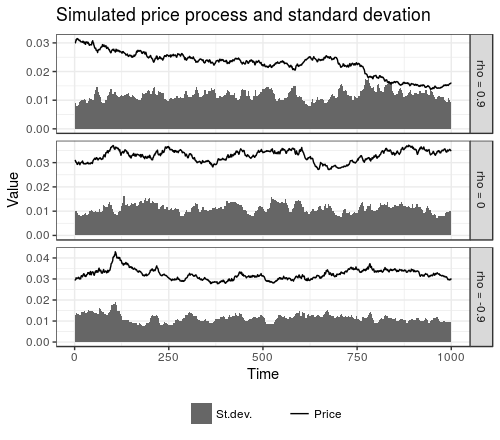
\includegraphics[width=\linewidth]{simulations/data-plot}
	\caption[Simulated price process and standard deviation]{Simulated price process scaled to 0.03 with its return's standard deviation. The relationship is visible: with high positive correlation (top) the price process and the volatility move together; with no correlation (middle) there is no visible pattern; with high negative correlation (bottom) the price process and the volatility move to the opposite direction.}
	\label{fig:simdata}
\end{figure}

\begin{figure}
	\centering
	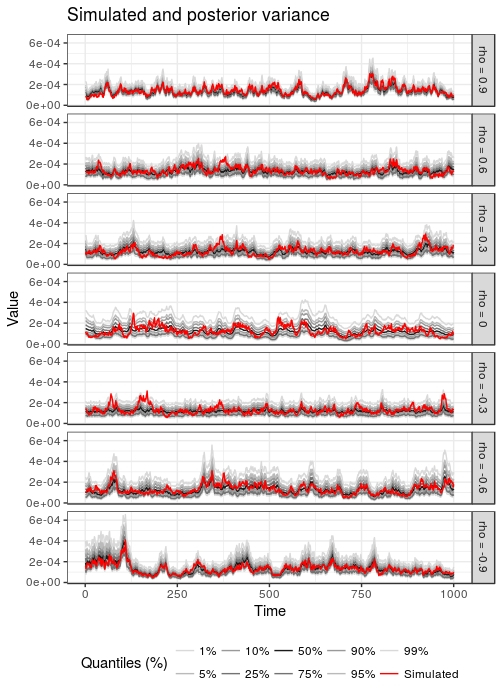
\includegraphics[width=\linewidth]{simulations/variance-plot}
	\caption{Simulated values and posterior quantiles of the variance process.}
	\label{fig:volatility}
\end{figure}

\begin{figure}
	\centering
	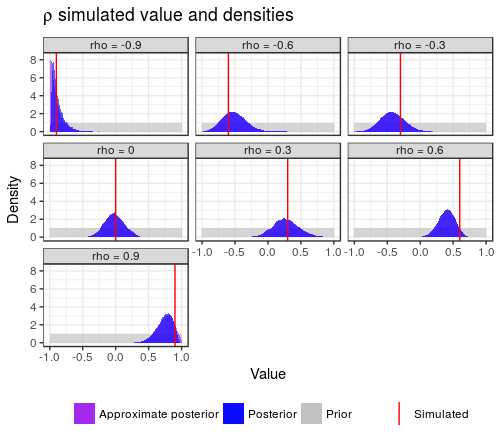
\includegraphics[width=\linewidth]{simulations/rho-densities}
	\caption[Prior, approximate and corrected posterior and simulated $\rho$]{Prior, approximate and corrected posterior distributions and the simulated value for $\rho$.}
	\label{fig:rhodensities}
\end{figure}

	\section{Empirical framework}

We would like to compare Chinese and German common stock's leverage effect independent of both time and company.
For that reason several stocks and time periods are chosen, and the model is fitted to each independently.
As a by-product, if it exists, the systematic time dependence of the leverage effect can be observed as well.

\subsection{Data}

Two stock indices served as starting points for the two countries: the SSE 50 Index from Shanghai for China, and the DAX Index from Frankfurt for Germany.
Then 10-10 companies were chosen randomly from the 50+30 currently listed ones such that they have a long enough stock price history, dating back to 2004.
Tables~\ref{tab:gercompanies} and~\ref{tab:chicompanies} show the final choice.
\begin{table}[h!]
	\centering
	\begin{tabular}{lr}
		\textbf{Company name} & \textbf{Bloomberg ticker} \\
		\hline
		BASF SE & BAS GY Equity \\
		Bayerische Motoren Werke AG & BMW GY Equity \\
		Commerzbank AG & CBK GY Equity \\
		Deutsche Telekom AG & DTE GY Equity \\
		HeidelbergCement AG & HEI GY Equity \\
		Linde AG & LIN GY Equity \\
		Merck KGaA & MRK GY Equity \\
		\thead[cl]{M\"unchener R\"uckversicherungs-\\\ Gesellschaft AG in M\"unchen} & MUV2 GY Equity \\
		SAP SE & SAP GY Equity \\
		Siemens AG & SIE GY Equity
	\end{tabular}
	\caption{German companies}
	\label{tab:gercompanies}
\end{table}

\begin{table}[h!]
	\centering
	\begin{tabular}{lr}
		\textbf{Company name} & \textbf{Bloomberg ticker} \\
		\hline
		\thead[cl]{Shanghai Pudong Development\\\ Bank Co., Ltd.} & 600000 CH Equity \\
		\thead[cl]{China Minsheng Bank} & 600016 CH Equity \\
		\thead[cl]{Citic Securities Co., Ltd.} & 600030 CH Equity \\
		\thead[cl]{China United Network\\\ Communications Ltd.} & 600050 CH Equity \\
		\thead[cl]{SAIC Motor Co., Ltd.} & 600104 CH Equity \\
		\thead[cl]{China Northern Rare Earth\\\ (Group) High-Tech Co., Ltd} & 600111 CH Equity \\
		\thead[cl]{China Fortune Land\\\ Development Co., Ltd.} & 600340 CH Equity \\
		\thead[cl]{Kweichow Moutai Co., Ltd.} & 600519 CH Equity \\
		\thead[cl]{Haitong Securities Co., Ltd} & 600837 CH Equity \\
		\thead[cl]{Inner Mongolia Yili\\\ Industrial Group Co., Ltd.} & 600887 CH Equity
	\end{tabular}
	\caption{Chinese companies}
	\label{tab:chicompanies}
\end{table}

Altogether 32 periods were used, all 3-year-long, in a moving window with step size of 3 months.
The first period is 2004/01/01-2006/12/31 and the last one 2011/10/01-2014/09/30.
This way the dataset fully includes the Subprime Crisis of 2007/08.

\subsection{Setup}

Almost the same prior distributions were used as in Section~\ref{sec:simulation}:
\begin{align*}
\frac{\phi+1}2 &\sim\text{Beta}(20,1.5), \\
\sigma^2 &\sim\text{InverseGamma}(2.25,\text{rate}=0.0625), \\
\rho &\sim\mathcal{U}(-1,1), \\
\mu &\sim\mathcal{N}(-9,1), \\
h_1\mid\phi,\sigma,\mu &\sim\mathcal{N}(\mu,\sigma^2/(1-\phi^2)).
\end{align*}
The only exception is $\sigma^2$, whose prior was copied from~\cite{Omori2007}.
In order to achieve convergence, a burn-in of 50,000 draws were used, and then $100\,000$ samples were recorded for evaluation, hence, a total of $20\times32\times(100\,000+50\,000)=96\,000\,000$ samples were drawn for data set sizes of around 750.

	\section{Results}

As it is shown in this section, our findings are mostly consistent with the literature.
In the examined period, among randomly chosen big corporations, the leverage effect in Germany is much stronger and sometimes the return-variance correlation is even positive in China.
Also, in general, the correlation shifted to the left throughout the crisis and its short term aftermath.

\subsection{Chinese anti-leverage}

Figure~\ref{fig:rhos} summarises all the results by plotting all the posterior densities obtained from the dataset.
Even though not all companies behave the same way, there is a consistent picture in general about the differences between the two countries.
The chart shows that, based on the chosen sample, $\rho$ is really estimated to be larger in China than in Germany, except for the periods containing the crisis, when it was similar.

The claims about China behaving differently are strengthened by Figure~\ref{fig:negative-rhos}, which shows the number of companies with a significant leverage or anti-leverage effect.
Interestingly, Germany had the least number of companies with significant leverage effect in the period that just preceded the crisis, which was followed by a steep increase in that number.
Apart from the periods containing the boom phase of the 2007 crisis or touching the European debt crisis, the Figure for Germany is quite stable around 6-7.
None of the German stocks had a significantly positive $\rho$.

The picture is much less consistent in China.
Ignoring periods with only one significant value, the leverage effect is only observed under the 2007 crisis with some delay compared to Germany, and only in 3 stocks at most, while anti-leverage is also only present before the crisis.
Still, the companies show some consistency, since there is not period with both leverage and anti-leverage effect being present.

Note that the exact distribution or point estimates of $\rho$ are not of high interest.
On the one hand, it is not the correlation of returns with variance changes but with log variance changes, which makes it more difficult to interpret.
On the other hand, comparison with correlation values obtained from other models in the literature is also not trivial, so across models only the sign and highly extreme values are interesting.

\subsection{Time dependence of leverage}

When time-variability is the question, comparison of $\rho$ estimates using the same model for different datasets can be helpful, and Figures~\ref{fig:rhos} and~\ref{fig:negative-rhos} suggest that leverage is not constant, not even its sign.
The charts show that correlation shifts to the negative direction in the crisis, which claim is consistent with recent literature~\citep{Christensen2015}.
It seems to hold especially for the Chinese stocks since the German companies are more stably on the negative side throughout the whole time.

Figure~\ref{fig:company-rhos} presents more details by showing how the posterior distribution changed with the rolling window of periods.
Indeed, the bottom half of the chart, the German companies are in general below zero since the crisis, showing a quite consistent picture.
BMW and SAP show a steadily strengthening leverage effect, the others either stagnate or show signs of end of the crisis, if we accept the hypothesis from~\citet{Christensen2015}, since the leverage effect is weakening in their case.

Each of the Chinese companies' show far more hectic time-dependence, but all had the negative extremum of the posteriors in a period containing the first half of 2008, at the strongest impact of the crisis.
However, in my view, the overall picture, being so unstable throughout the whole examined time, questions the reliability of the results from the perspective of~\citet{Christensen2015}.
There might be far more and a lot different factors in play that affect Chinese stocks' leverage effect.

\subsection{Volatility estimations}

The posterior of $\phi$ and of the log variance are presented in Figure~\ref{fig:persistence} on a chosen subset of periods and companies that represent the whole dataset.
The prior of $\phi$ is taken to be informative, it reflects the empirical fact of highly autocorrelating volatility, which is supposed to improve on convergence of the MCMC method.
The posterior of $\phi$ mainly depends on its prior and the estimate for $\bm h$, hence if the posterior is significantly different from the prior, that means that there is valuable information in $\bm h$ about $\phi$.

An immediately noticeable phenomenon on Figure~\ref{fig:persistence} is that the posterior of $\phi$ varies more for the German firms, or more precisely, throughout the crisis and in its short aftermath the volatility of the German stocks was much more persistent than in the other periods.
At the same time, changes in the persistence of the Chinese companies can not be explained by the crisis periods, and the estimates are more stable and closer to the prior, except for the highly persistent 2010-2012 period of 600016 CH Equity.
One can also spot the differences on the log variance timeline: the time series are close to a constant value plus noise in China, containing little information about persistence, contrary to Germany, where clusters of increasing and decreasing trends can be observed around the crisis.

\begin{figure}[p]
	\vspace*{-3.2cm}
	\centering
	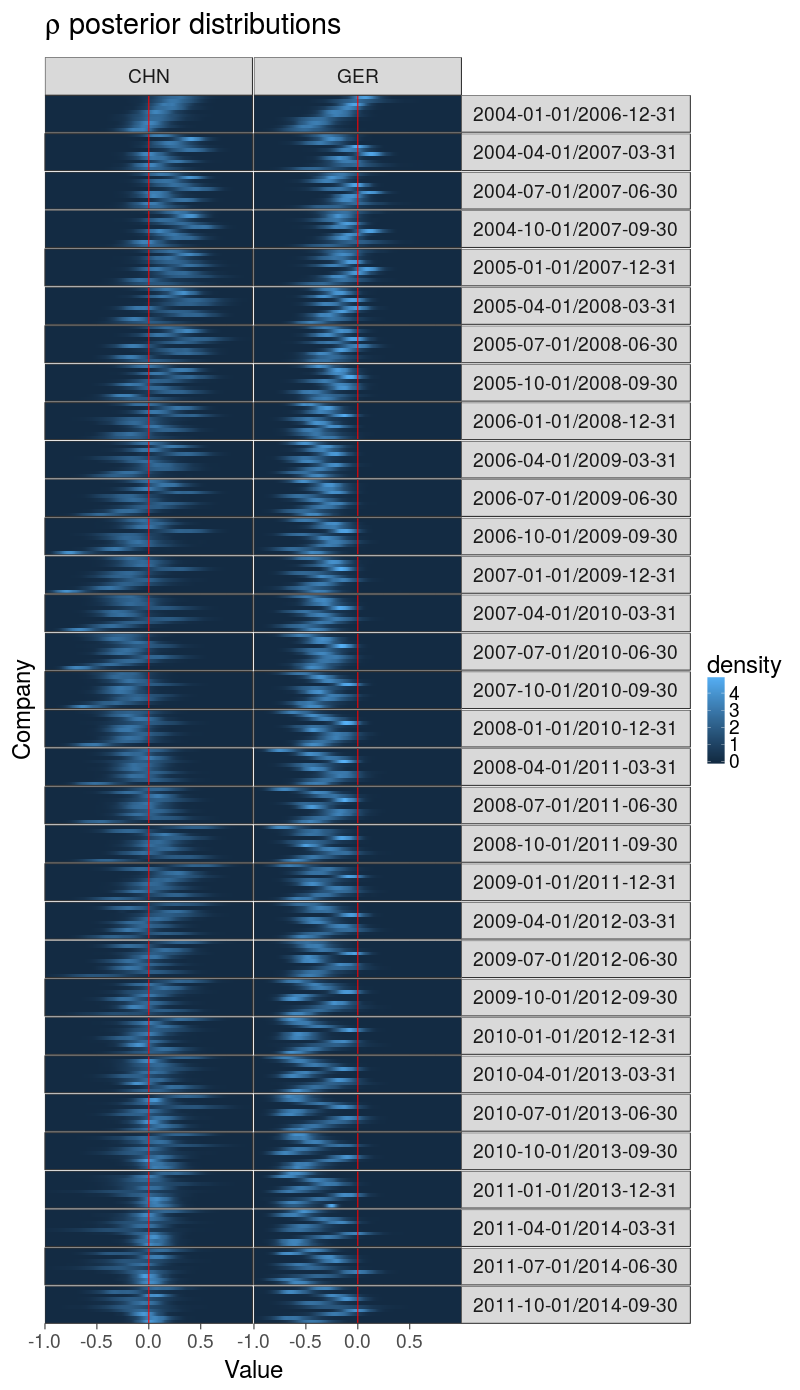
\includegraphics[width=\linewidth]{../calculations/rhos.pdf}
	\caption[Visually summarising all results]{Visually summarising all results. Each blue box corresponds to a country and a period and contains 10 rows. One row corresponds to one stock. Each row is a heatmap of $\rho$'s posterior density estimated for that company and period. The red line is constant 0. The stocks' rows are ordered according to their posterior mean in the first period.}
	\label{fig:rhos}
\end{figure}

\begin{figure}[p]
	\vspace*{-3.2cm}
	\centering
	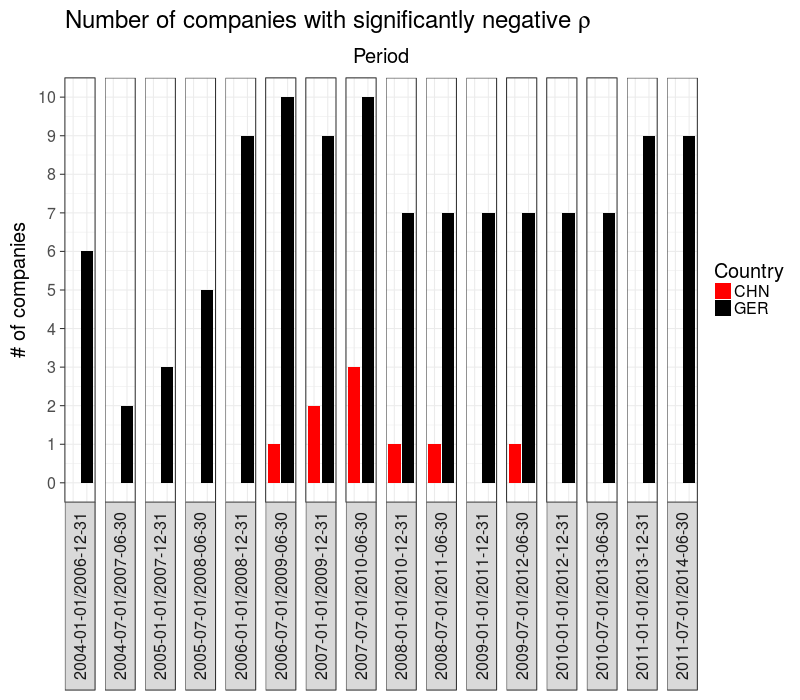
\includegraphics[width=\linewidth]{../calculations/negative-rhos.pdf}
	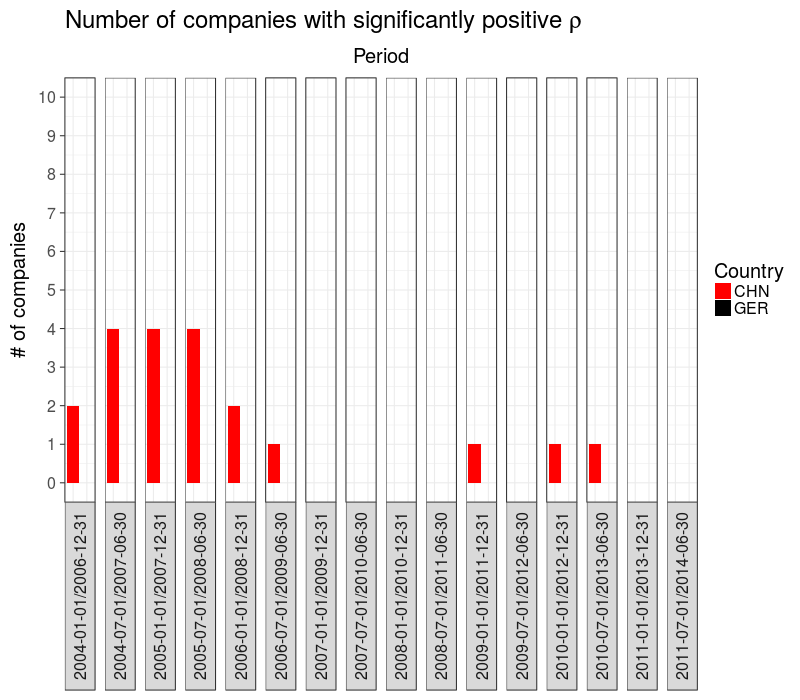
\includegraphics[width=\linewidth]{../calculations/positive-rhos.pdf}
	\caption[Significant leverage effect]{Top: number of companies with significant leverage effect per country and period, on a 5\% level. Bottom: number of companies with significant anti-leverage effect per country and period, on a 5\% level. Both: Only every second period is shown for readability.}
	\label{fig:negative-rhos}
\end{figure}

\begin{figure}[p]
	\vspace*{-3.2cm}
	\centering
	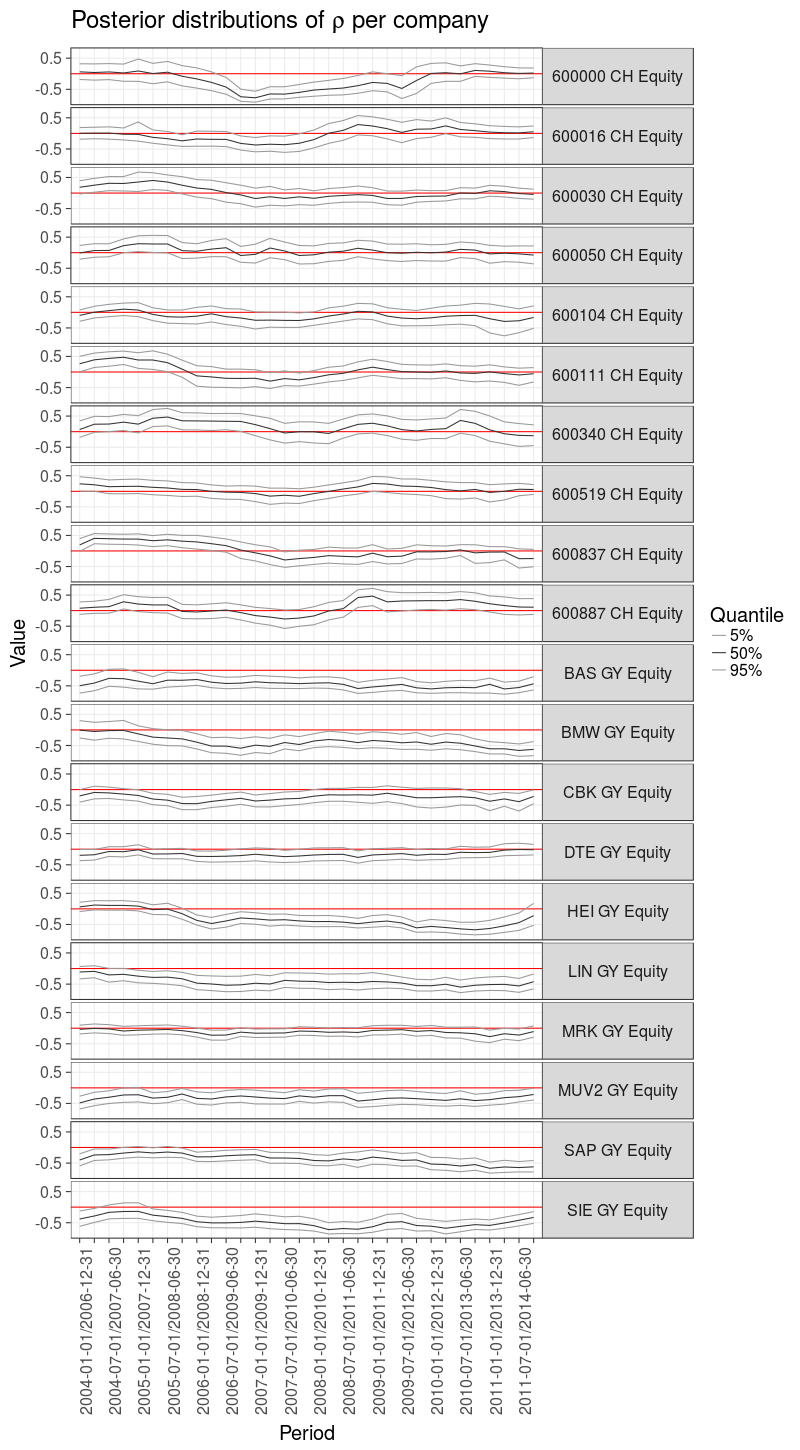
\includegraphics[width=\linewidth]{../calculations/rho-timeline.pdf}
	\caption[Timeline of posterior $\rho$]{Posterior distributions of $\rho$ in time. The prior distribution is the standard uniform in all cases.}
	\label{fig:company-rhos}
\end{figure}

\begin{figure}[p]
	\vspace*{-3.2cm}
	\centering
	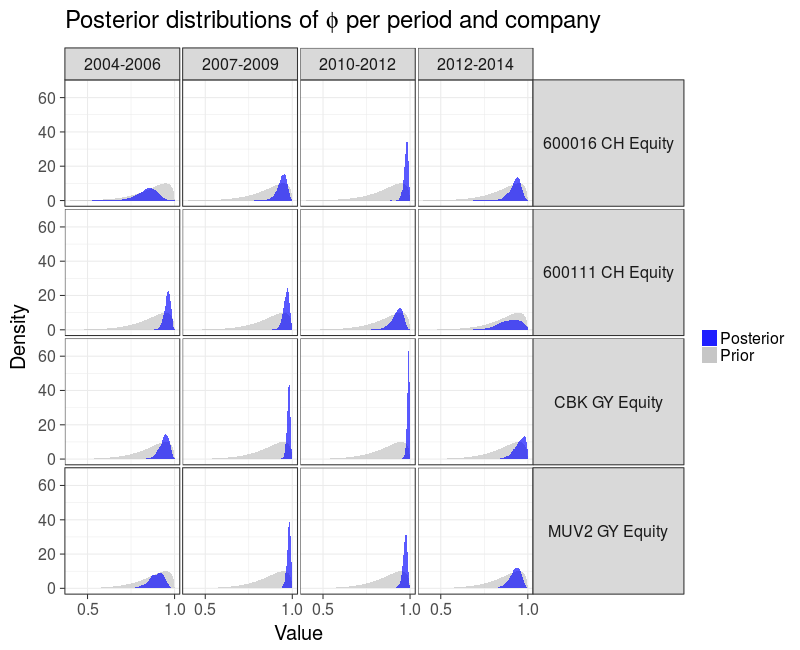
\includegraphics[width=\linewidth]{../calculations/phi-timeline.pdf}
	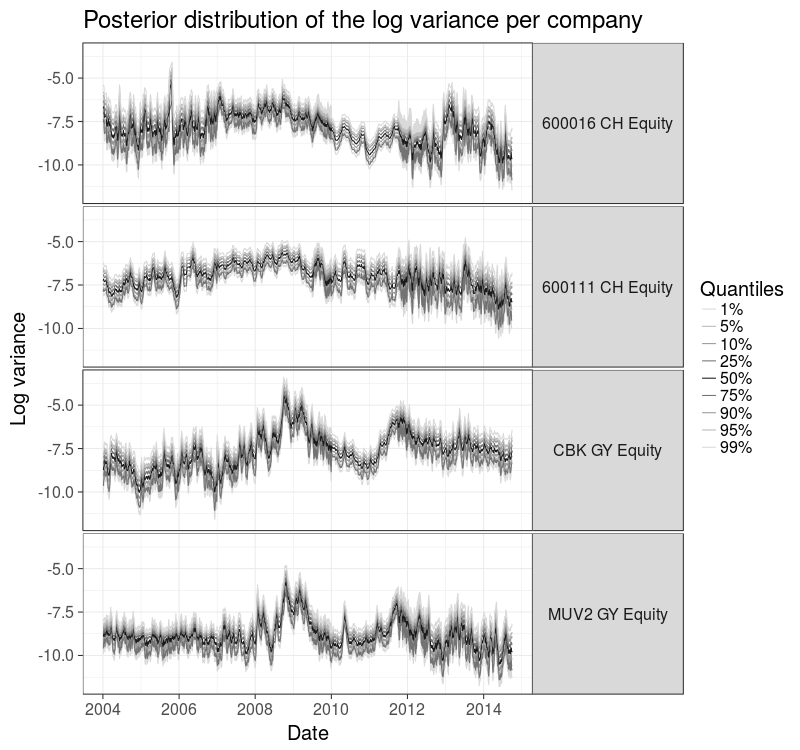
\includegraphics[width=\linewidth]{../calculations/volatility.pdf}
	\caption[Timeline of persistence and volatility]{Top: posterior persistence of the log variance for a subset of companies and periods. Bottom: posterior log variance for a subset of the companies. The time series are glued together from the independent volatility estimations from several periods.}
	\label{fig:persistence}
\end{figure}

	\section{Conclusion}

The main research question is whether, based on our observations, Chinese stocks showed a positive return-variance correlation.
That we cannot claim in general since in all periods more than half of the Chinese companies' $\rho$ estimate was not significantly different from 0.
On the other hand, what we can say is that, outside of the deepest times of the 2007 crisis, the Chinese market participants uniformly show weaker leverage effect than the German ones, most of the times an insignificant one, sometimes they even show anti-leverage.

Examining further differences and similarities is most interesting with the global crisis of 2007 in mind.
We found proof for $\rho$ being shifted to the negative direction throughout the crisis contained by the sample.
That behaviour was present unquestionably in both countries, although the hectic changes of the leverage effect in China bring doubts about the importance of the crisis as a driving factor for them.

While $\rho$ does not necessarily do, estimates of $\phi$ separate the two countries.
When there is a trend in the volatility, i.e.\ it is not constant plus white noise, then there is high autocorrelation and persistence.
These trends exist in the German stocks' volatilities around the Subprime Crisis and the European Debt Crisis, at those times $\phi$ is significantly larger than its prior, while this phenomenon is not present in China.

\subsection{Future work}

While there are many possible explanations for the leverage effect, there is not any for the anti-leverage effect, to the best of our knowledge.
Unusual regulations are likely to be the main factor here, or a different investment culture.
Either way, a microeconomics-based approach could be the key that models agents maximising utility in a well designed environment.

Finally, time-varying leverage effect models could be another direction for improvements.
Simple linear functions would not be sufficient to model the shifts in crises, probably a higher order polynomial that still avoids overfitting, or an ARCH process for $\rho$ would increase the predictive power.
We did not find such attempts in the literature.


	
	%\nocite{*}
	\bibliographystyle{abbrvnat}
	\bibliography{references}
	
\end{document}
